% Options for packages loaded elsewhere
\PassOptionsToPackage{unicode}{hyperref}
\PassOptionsToPackage{hyphens}{url}
\PassOptionsToPackage{dvipsnames,svgnames,x11names}{xcolor}
%
\documentclass[
  ignorenonframetext,
]{beamer}
\usepackage{pgfpages}
\setbeamertemplate{caption}[numbered]
\setbeamertemplate{caption label separator}{: }
\setbeamercolor{caption name}{fg=normal text.fg}
\beamertemplatenavigationsymbolsempty
% Prevent slide breaks in the middle of a paragraph
\widowpenalties 1 10000
\raggedbottom

\usepackage{amsmath,amssymb}
\usepackage{iftex}
\ifPDFTeX
  \usepackage[T1]{fontenc}
  \usepackage[utf8]{inputenc}
  \usepackage{textcomp} % provide euro and other symbols
\else % if luatex or xetex
  \usepackage{unicode-math}
  \defaultfontfeatures{Scale=MatchLowercase}
  \defaultfontfeatures[\rmfamily]{Ligatures=TeX,Scale=1}
\fi
\usepackage{lmodern}
\usetheme[]{AnnArbor}
\usecolortheme{dolphin}
\usefonttheme{structurebold}
\ifPDFTeX\else  
    % xetex/luatex font selection
\fi
% Use upquote if available, for straight quotes in verbatim environments
\IfFileExists{upquote.sty}{\usepackage{upquote}}{}
\IfFileExists{microtype.sty}{% use microtype if available
  \usepackage[]{microtype}
  \UseMicrotypeSet[protrusion]{basicmath} % disable protrusion for tt fonts
}{}
\makeatletter
\@ifundefined{KOMAClassName}{% if non-KOMA class
  \IfFileExists{parskip.sty}{%
    \usepackage{parskip}
  }{% else
    \setlength{\parindent}{0pt}
    \setlength{\parskip}{6pt plus 2pt minus 1pt}}
}{% if KOMA class
  \KOMAoptions{parskip=half}}
\makeatother
\usepackage{xcolor}
\newif\ifbibliography
\setlength{\emergencystretch}{3em} % prevent overfull lines
\setcounter{secnumdepth}{-\maxdimen} % remove section numbering


\providecommand{\tightlist}{%
  \setlength{\itemsep}{0pt}\setlength{\parskip}{0pt}}\usepackage{longtable,booktabs,array}
\usepackage{calc} % for calculating minipage widths
\usepackage{caption}
% Make caption package work with longtable
\makeatletter
\def\fnum@table{\tablename~\thetable}
\makeatother
\usepackage{graphicx}
\makeatletter
\def\maxwidth{\ifdim\Gin@nat@width>\linewidth\linewidth\else\Gin@nat@width\fi}
\def\maxheight{\ifdim\Gin@nat@height>\textheight\textheight\else\Gin@nat@height\fi}
\makeatother
% Scale images if necessary, so that they will not overflow the page
% margins by default, and it is still possible to overwrite the defaults
% using explicit options in \includegraphics[width, height, ...]{}
\setkeys{Gin}{width=\maxwidth,height=\maxheight,keepaspectratio}
% Set default figure placement to htbp
\makeatletter
\def\fps@figure{htbp}
\makeatother
% definitions for citeproc citations
\NewDocumentCommand\citeproctext{}{}
\NewDocumentCommand\citeproc{mm}{%
  \begingroup\def\citeproctext{#2}\cite{#1}\endgroup}
\makeatletter
 % allow citations to break across lines
 \let\@cite@ofmt\@firstofone
 % avoid brackets around text for \cite:
 \def\@biblabel#1{}
 \def\@cite#1#2{{#1\if@tempswa , #2\fi}}
\makeatother
\newlength{\cslhangindent}
\setlength{\cslhangindent}{1.5em}
\newlength{\csllabelwidth}
\setlength{\csllabelwidth}{3em}
\newenvironment{CSLReferences}[2] % #1 hanging-indent, #2 entry-spacing
 {\begin{list}{}{%
  \setlength{\itemindent}{0pt}
  \setlength{\leftmargin}{0pt}
  \setlength{\parsep}{0pt}
  % turn on hanging indent if param 1 is 1
  \ifodd #1
   \setlength{\leftmargin}{\cslhangindent}
   \setlength{\itemindent}{-1\cslhangindent}
  \fi
  % set entry spacing
  \setlength{\itemsep}{#2\baselineskip}}}
 {\end{list}}
\usepackage{calc}
\newcommand{\CSLBlock}[1]{\hfill\break\parbox[t]{\linewidth}{\strut\ignorespaces#1\strut}}
\newcommand{\CSLLeftMargin}[1]{\parbox[t]{\csllabelwidth}{\strut#1\strut}}
\newcommand{\CSLRightInline}[1]{\parbox[t]{\linewidth - \csllabelwidth}{\strut#1\strut}}
\newcommand{\CSLIndent}[1]{\hspace{\cslhangindent}#1}

\usepackage{booktabs}
\usepackage{longtable}
\usepackage{array}
\usepackage{multirow}
\usepackage{wrapfig}
\usepackage{float}
\usepackage{colortbl}
\usepackage{pdflscape}
\usepackage{tabu}
\usepackage{threeparttable}
\usepackage{threeparttablex}
\usepackage[normalem]{ulem}
\usepackage{makecell}
\usepackage{xcolor}

% logo
\titlegraphic{
\includegraphics[width=4cm]{000_logos/logo-blue-vertical}}
\logo{\ifnum\thepage>1
\includegraphics[width=0.5cm]{000_logos/logo-blue-vertical}\fi}

% UMNG: Manual de image institucional

% Colors

% Umng
\definecolor{yellow}{HTML}{fdc600}
\definecolor{red}{HTML}{ee2a24}

% Estudios a Distancia
\definecolor{blue1}{HTML}{12245b}
\definecolor{blue2}{HTML}{767ca6}
\definecolor{blue3}{HTML}{cad2ec}

% Modify items
\setbeamercolor{palette primary}{bg=blue3}
\setbeamercolor{palette tertiary}{bg=blue1}
\setbeamercolor{frametitle}{bg=yellow}

% Hyperlinks
\hypersetup{
  linkcolor=red,
  citecolor=red
}

\makeatletter
\@ifpackageloaded{caption}{}{\usepackage{caption}}
\AtBeginDocument{%
\ifdefined\contentsname
  \renewcommand*\contentsname{Table of contents}
\else
  \newcommand\contentsname{Table of contents}
\fi
\ifdefined\listfigurename
  \renewcommand*\listfigurename{List of Figures}
\else
  \newcommand\listfigurename{List of Figures}
\fi
\ifdefined\listtablename
  \renewcommand*\listtablename{List of Tables}
\else
  \newcommand\listtablename{List of Tables}
\fi
\ifdefined\figurename
  \renewcommand*\figurename{Figure}
\else
  \newcommand\figurename{Figure}
\fi
\ifdefined\tablename
  \renewcommand*\tablename{Table}
\else
  \newcommand\tablename{Table}
\fi
}
\@ifpackageloaded{float}{}{\usepackage{float}}
\floatstyle{ruled}
\@ifundefined{c@chapter}{\newfloat{codelisting}{h}{lop}}{\newfloat{codelisting}{h}{lop}[chapter]}
\floatname{codelisting}{Listing}
\newcommand*\listoflistings{\listof{codelisting}{List of Listings}}
\makeatother
\makeatletter
\makeatother
\makeatletter
\@ifpackageloaded{caption}{}{\usepackage{caption}}
\@ifpackageloaded{subcaption}{}{\usepackage{subcaption}}
\makeatother

\ifLuaTeX
\usepackage[bidi=basic]{babel}
\else
\usepackage[bidi=default]{babel}
\fi
\babelprovide[main,import]{english}
% get rid of language-specific shorthands (see #6817):
\let\LanguageShortHands\languageshorthands
\def\languageshorthands#1{}
\ifLuaTeX
  \usepackage{selnolig}  % disable illegal ligatures
\fi
\usepackage{bookmark}

\IfFileExists{xurl.sty}{\usepackage{xurl}}{} % add URL line breaks if available
\urlstyle{same} % disable monospaced font for URLs
\hypersetup{
  pdftitle={Economic Growth},
  pdfauthor={Luis Francisco Gómez López},
  pdflang={en},
  colorlinks=true,
  linkcolor={Maroon},
  filecolor={Maroon},
  citecolor={Blue},
  urlcolor={Blue},
  pdfcreator={LaTeX via pandoc}}


\title{Economic Growth}
\author{Luis Francisco Gómez López}
\date{2024-07-14}
\institute{FAEDIS}

\begin{document}
\frame{\titlepage}

\renewcommand*\contentsname{Table of contents}
\begin{frame}[allowframebreaks]
  \frametitle{Table of contents}
  \tableofcontents[hideallsubsections]
\end{frame}

\section{Please Read Me}\label{please-read-me}

\begin{frame}{}
\phantomsection\label{section}
\begin{itemize}
\item
  Check the message \textbf{Welcome greeting} published in the News
  Bulletin Board.
\item
  Dear student please edit your profile uploading a photo where your
  face is clearly visible.
\item
  The purpose of the virtual meetings is to answer questions and not to
  make a summary of the study material.
\item
  This presentation is based on
  (\citeproc{ref-cardenas_introduccion_2020}{Cardenas 2020, chap. 3})
\end{itemize}
\end{frame}

\section{Purpose}\label{purpose}

\begin{frame}{}
\phantomsection\label{section-1}
Analyze the determinants of economic growth
\end{frame}

\section{What is economic growth?}\label{what-is-economic-growth}

\begin{frame}{}
\phantomsection\label{section-2}
\begin{itemize}
\item
  Economic growth can be define as an increase in the quantity and
  quality of products that a society produces and consumes
  (\citeproc{ref-roser_economic_2013}{Roser 2013})
\item
  The definition of economic growth is straightforward but this concept
  is extremely difficult to measure
  (\citeproc{ref-roser_economic_2013}{Roser 2013})
\item
  Economists often measure economic growth as an increase in Gross
  Domestic Product per capita by applying inflation adjustments.
  Furthermore, if international comparisons are necessary also purchase
  power parity (PPP) adjustments are applied
  (\citeproc{ref-roser_economic_2013}{Roser 2013})
\item
  From the long-term perspective of social history economic growth is a
  recent phenomena (\citeproc{ref-roser_economic_2013}{Roser 2013})
\item
  For data related to economic growth from a long-term perspective check
  out (\citeproc{ref-bolt_maddisonstyle_2024}{Bolt and Van Zanden
  2024b}) and (\citeproc{ref-bolt_maddison_2024}{Bolt and Van Zanden
  2024a})
\end{itemize}
\end{frame}

\section{Economic growth from a long-term
perspective}\label{economic-growth-from-a-long-term-perspective}

\begin{frame}{}
\phantomsection\label{section-3}
\begin{figure}

\centering{

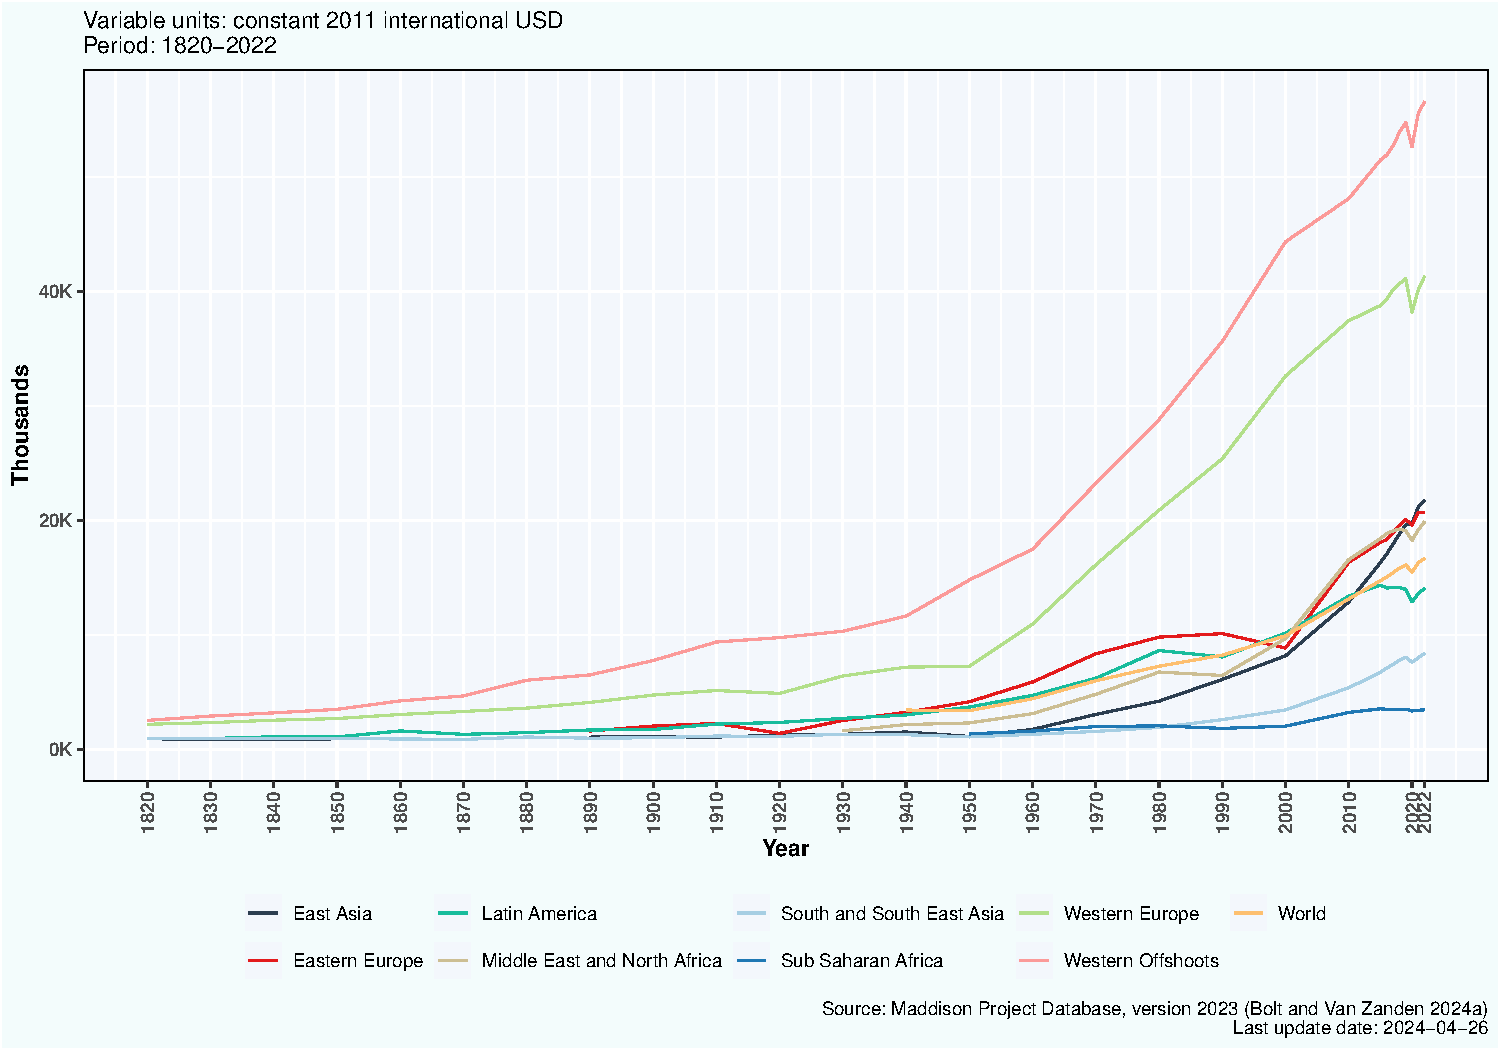
\includegraphics[width=0.85\textwidth,height=\textheight]{003_economic_growth_files/figure-beamer/fig-gdp-pc-ppp-latin-america-world-1.pdf}

}

\caption{\label{fig-gdp-pc-ppp-latin-america-world}GDP per−capita
purchasing power parity, Latin America and the World}

\end{figure}%
\end{frame}

\section{Economic growth paths}\label{economic-growth-paths}

\begin{frame}{}
\phantomsection\label{section-4}
\begin{figure}

\centering{

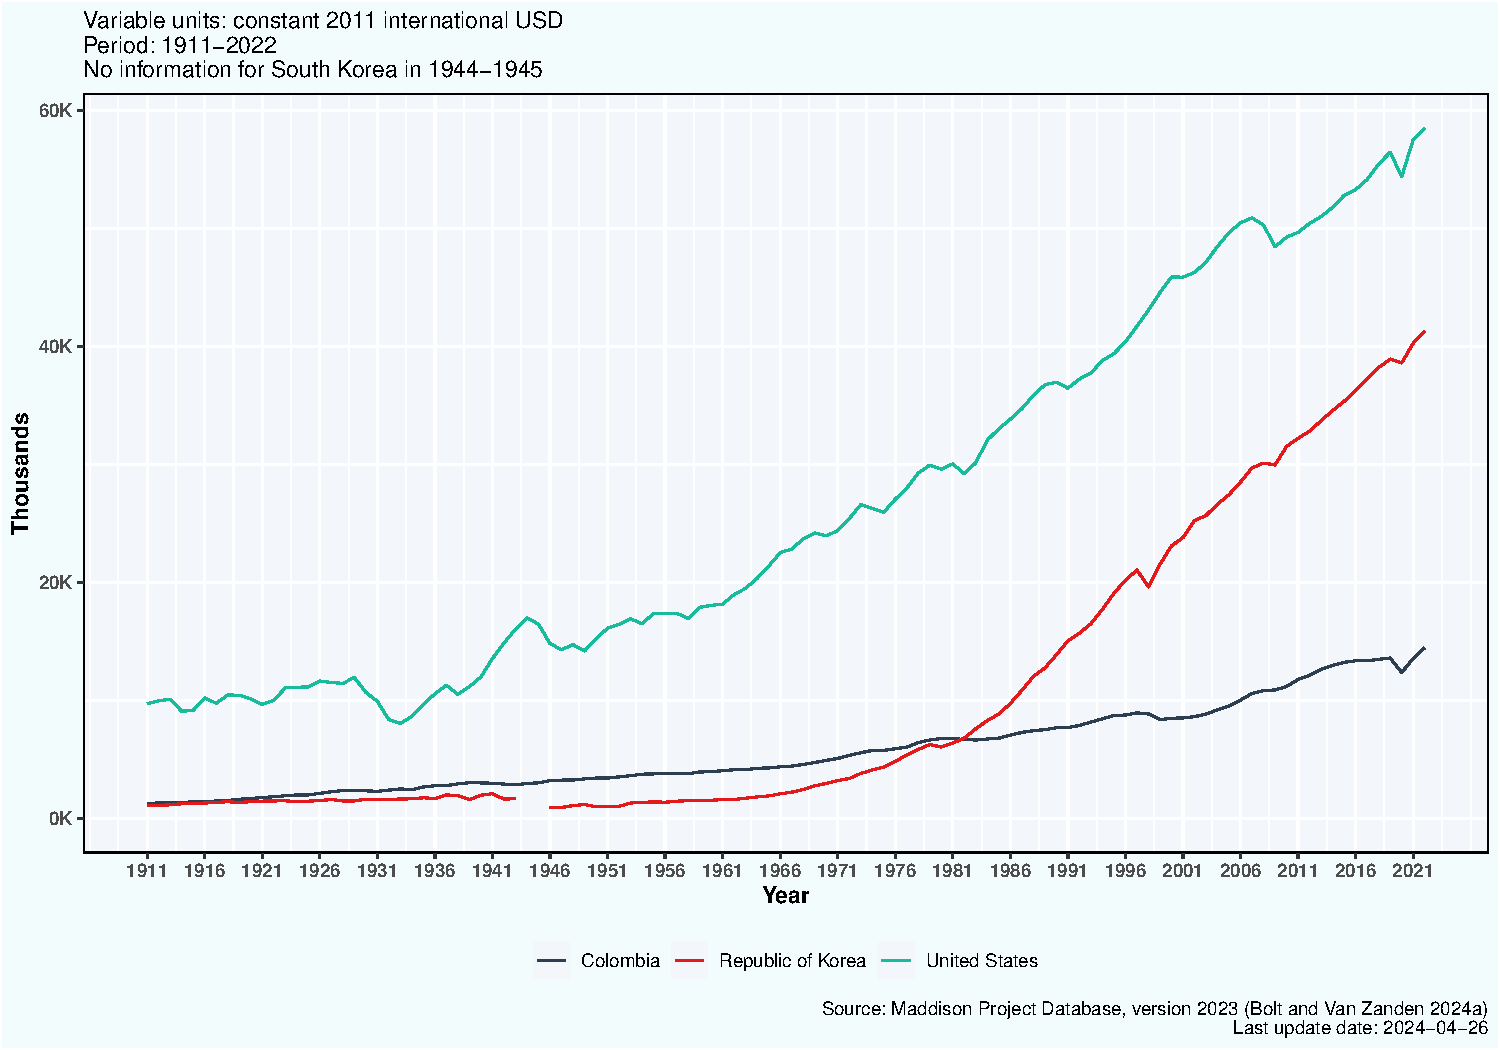
\includegraphics[width=0.85\textwidth,height=\textheight]{003_economic_growth_files/figure-beamer/fig-growth-paths-usa-col-kor-1.pdf}

}

\caption{\label{fig-growth-paths-usa-col-kor}GDP per-capita purchasing
power parity, Colombia, USA and South Korea}

\end{figure}%
\end{frame}

\begin{frame}{}
\phantomsection\label{section-5}
\begin{figure}

\centering{

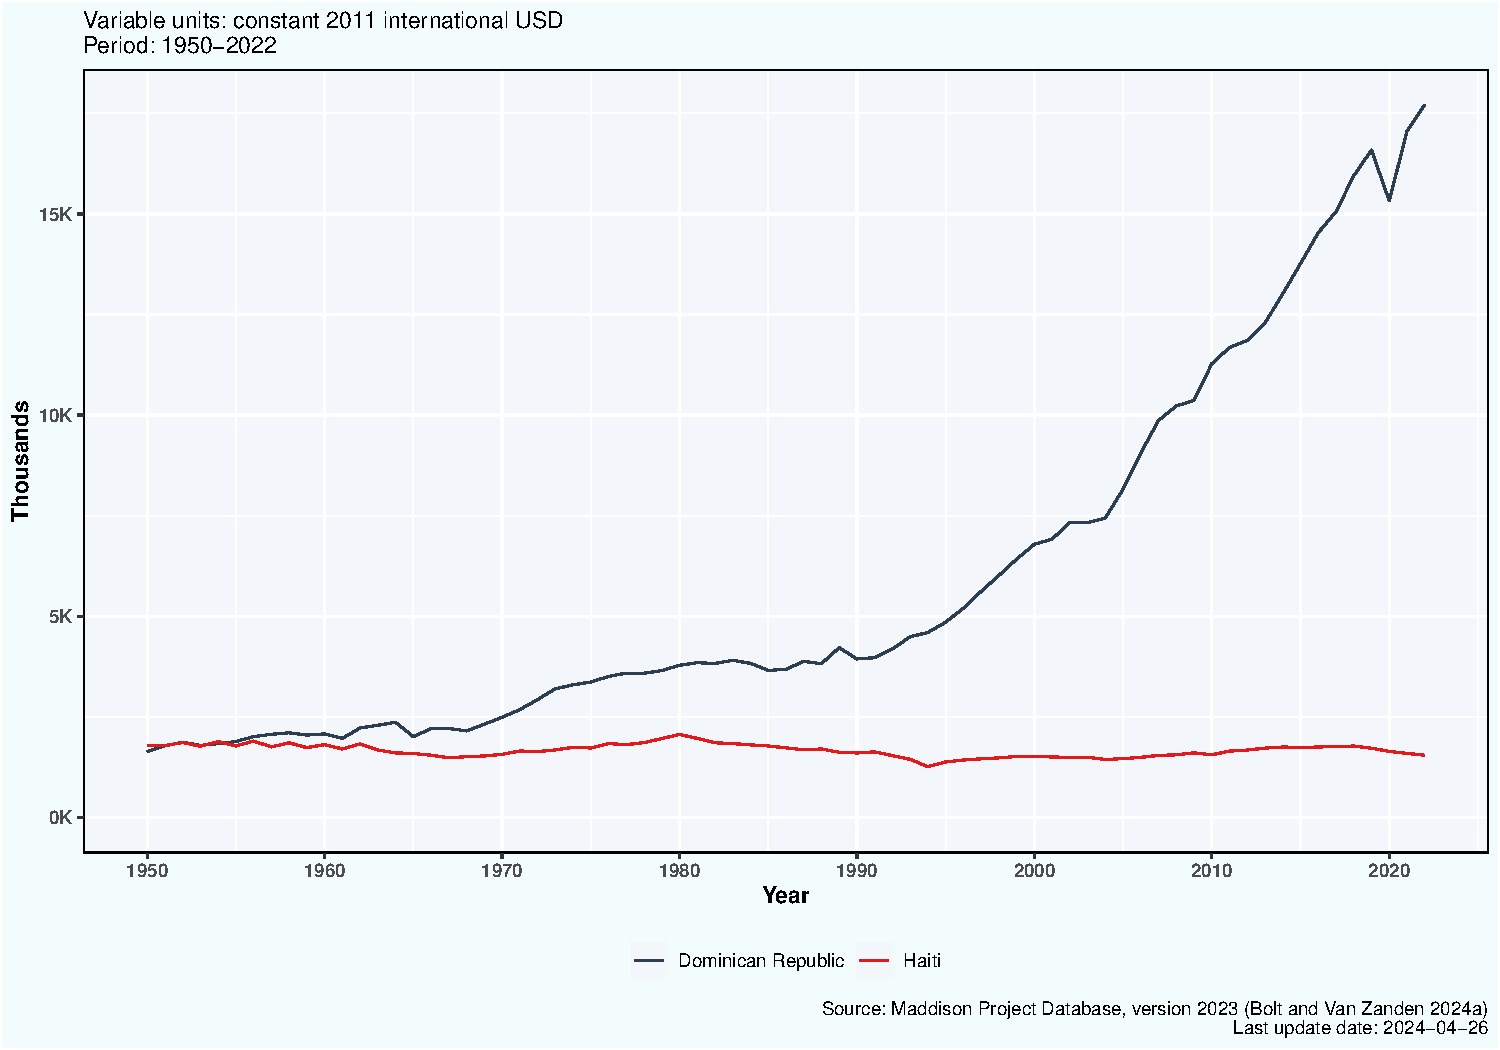
\includegraphics[width=0.85\textwidth,height=\textheight]{003_economic_growth_files/figure-beamer/fig-growth-paths-hti-dom-1.pdf}

}

\caption{\label{fig-growth-paths-hti-dom}GDP per-capita purchasing power
parity, Haiti and Dominican Republic}

\end{figure}%
\end{frame}

\begin{frame}{}
\phantomsection\label{section-6}
\begin{figure}

\centering{

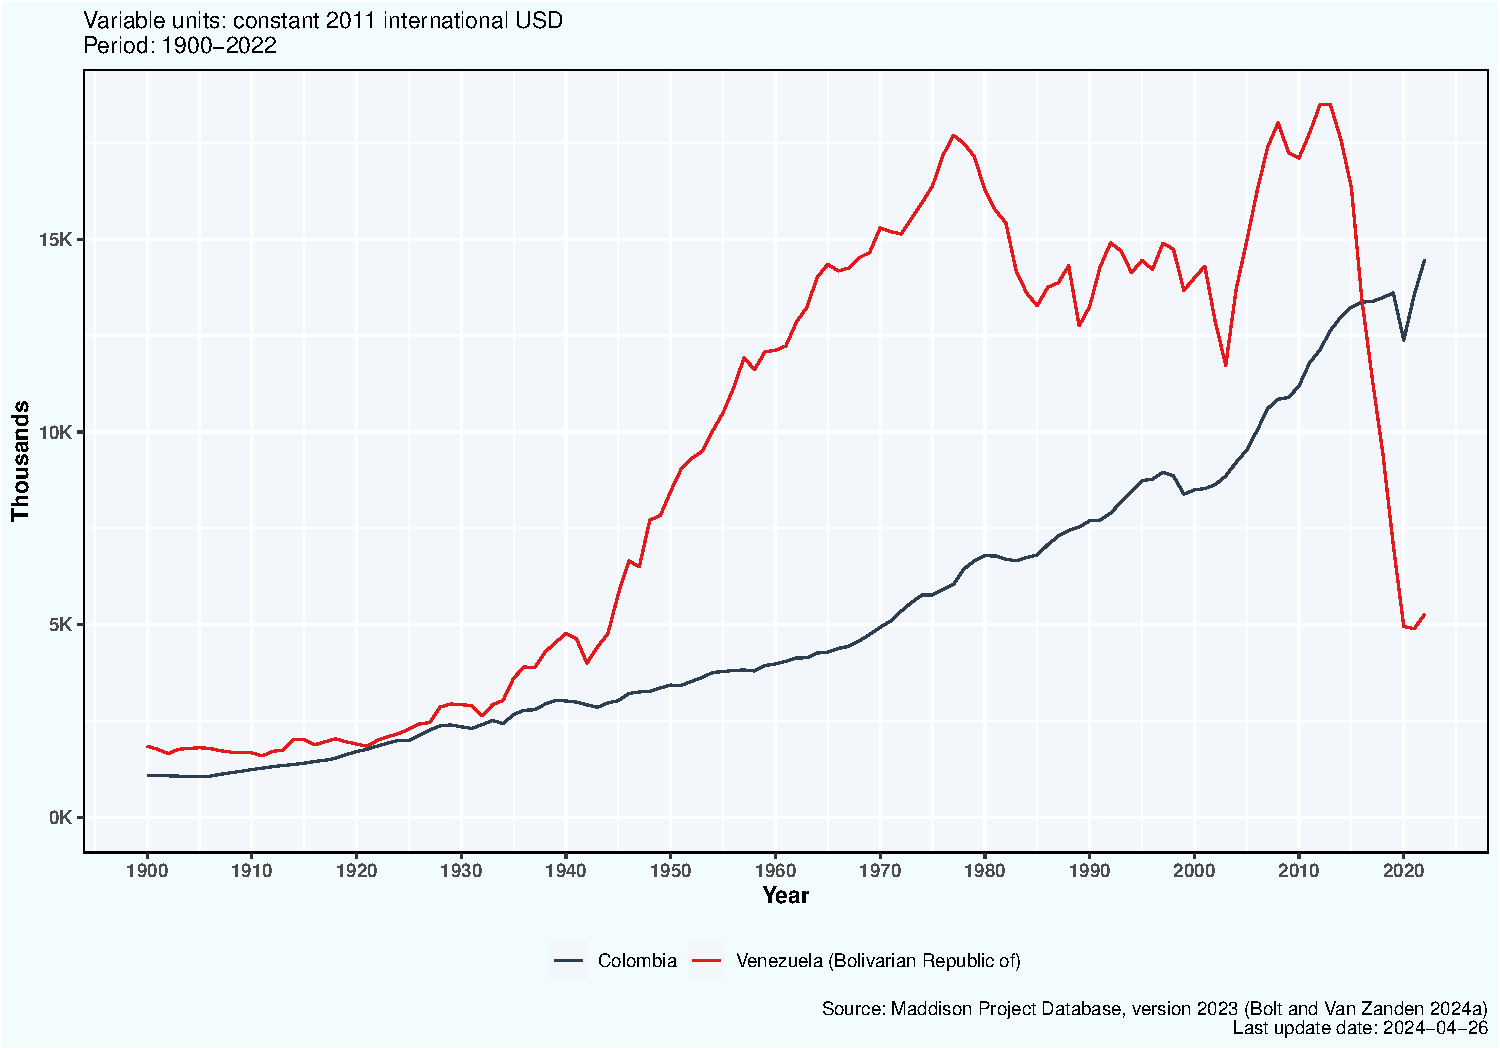
\includegraphics[width=0.85\textwidth,height=\textheight]{003_economic_growth_files/figure-beamer/fig-growth-paths-col-ven-1.pdf}

}

\caption{\label{fig-growth-paths-col-ven}GDP per-capita purchasing power
parity, Colombia and Venezuela}

\end{figure}%
\end{frame}

\section{Economic growth in images}\label{economic-growth-in-images}

\begin{frame}{}
\phantomsection\label{section-7}
\begin{figure}

\begin{minipage}{0.50\linewidth}

\centering{

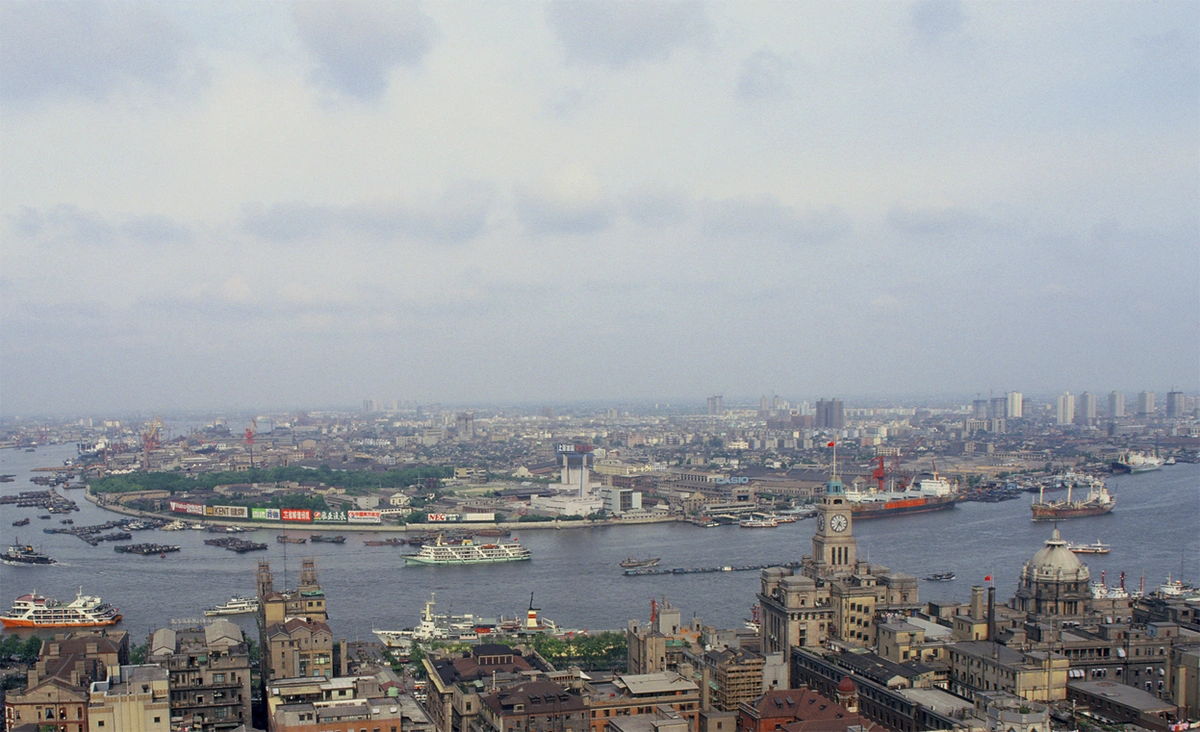
\includegraphics[width=2.1875in,height=2.1875in]{_000_images/003_pudong_1987.png}

}

\subcaption{\label{fig-pudong-1987}1987}

\end{minipage}%
%
\begin{minipage}{0.50\linewidth}

\centering{

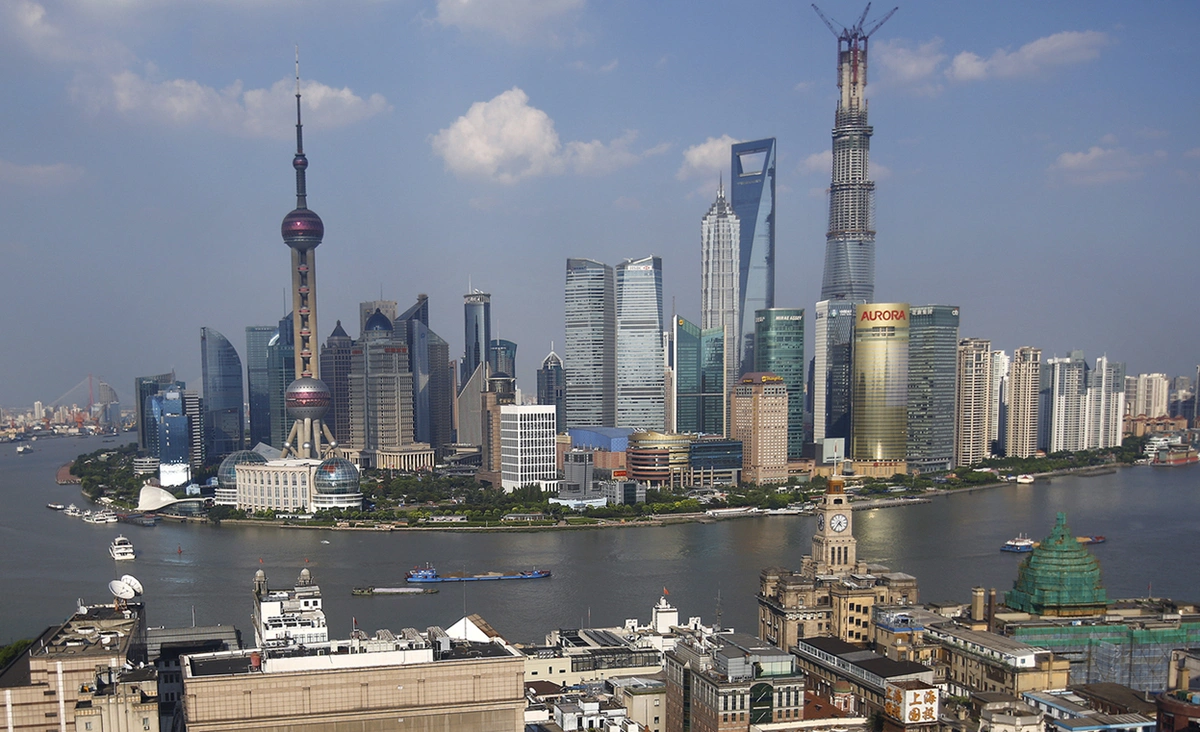
\includegraphics[width=2.1875in,height=2.1875in]{_000_images/003_pudong_2013.png}

}

\subcaption{\label{fig-pudong-2013}2013}

\end{minipage}%

\caption{\label{fig-shangai_financial_district_pudong}Shanghai's
financial district of Pudong (\citeproc{ref-taylor_26_2013}{Taylor
2013})}

\end{figure}%
\end{frame}

\begin{frame}{}
\phantomsection\label{section-8}
\begin{figure}

\centering{

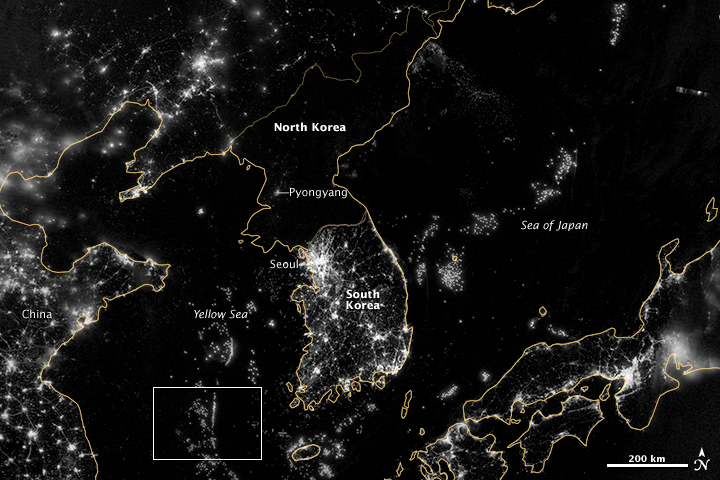
\includegraphics[width=3.64583in,height=3.64583in]{_000_images/003_north_south_koreas.png}

}

\caption{\label{fig-korean-peninsula-nocturnal-luminosity}Korean
peninsula, nocturnal luminosity: September 24, 2012
(\citeproc{ref-nasa_earth_observatory_korea_2012}{Observatory, Allen,
and Simmon 2012})}

\end{figure}%
\end{frame}

\begin{frame}{}
\phantomsection\label{section-9}
\begin{itemize}
\item
  Google Earth Timelapse Dubai, UAE check out\footnote<.->{Timelapse is
    a global, zoomable video that lets you see how the Earth has changed
    over the past 32 years.}:

  \begin{itemize}
  \tightlist
  \item
    \url{https://youtu.be/pjM26oRIay0}
  \end{itemize}
\item
  Explore about Timelapse at:
  \url{https://earthengine.google.com/timelapse}

  \begin{itemize}
  \item
    Urban growth

    \begin{itemize}
    \tightlist
    \item
      Dalian, Liaoning, China
    \item
      Las Vegas, Nevada, USA
    \end{itemize}
  \end{itemize}
\end{itemize}
\end{frame}

\section{Inputs to obtain GDP}\label{inputs-to-obtain-gdp}

\begin{frame}{}
\phantomsection\label{section-10}
Gross domestic product is obtained by using the following inputs:

\begin{itemize}
\item
  Labor

  \begin{itemize}
  \tightlist
  \item
    Quantity of labor:

    \begin{itemize}
    \tightlist
    \item
      Employment\footnote<.->{Includes individuals employed aged 15
        years or over where this age range is necessary for
        international comparisons.}
    \item
      Hours worked
    \end{itemize}
  \item
    Quality of Labor:

    \begin{itemize}
    \tightlist
    \item
      Employment by educational attainment
    \item
      Compensation by educational attainment
    \end{itemize}
  \end{itemize}
\end{itemize}
\end{frame}

\begin{frame}{}
\phantomsection\label{section-11}
Gross domestic product is obtained by using the following inputs:

\begin{itemize}
\item
  Produced non-financial fixed assets\footnote<.->{Other non-financial
    assets can be included but these are the ones that are usually
    measured. For more information check out
    (\citeproc{ref-oecd_measuring_2009}{OECD 2009}) and
    (\citeproc{ref-oecd_measuring_2001}{OECD 2001})}

  \begin{itemize}
  \tightlist
  \item
    Dwellings
  \item
    Buildings other than dwellings
  \item
    Other structures
  \item
    Land improvements
  \item
    Transport equipment
  \item
    Information and Computer Technology (ICT) equipment
  \item
    Other machinery and equipment
  \item
    Weapons systems
  \item
    Cultivated biological resources
  \end{itemize}
\end{itemize}
\end{frame}

\begin{frame}{}
\phantomsection\label{section-12}
Other factors that affect the Gross Domestic Product different from
labor and produced non-financial fixed assets

\begin{itemize}
\item
  These factors are not directly observable but are used in growth
  accounting to calculate \textbf{Total Factor Productivity/Multifactor
  productivity} as an approximation to technological change

  \begin{itemize}
  \tightlist
  \item
    Technological change is defined as changes in the Gross Domestic
    Product that are not due to changes in inputs
  \end{itemize}
\end{itemize}
\end{frame}

\section{Growth accounting}\label{growth-accounting}

\begin{frame}{}
\phantomsection\label{section-13}
\begin{figure}

\centering{

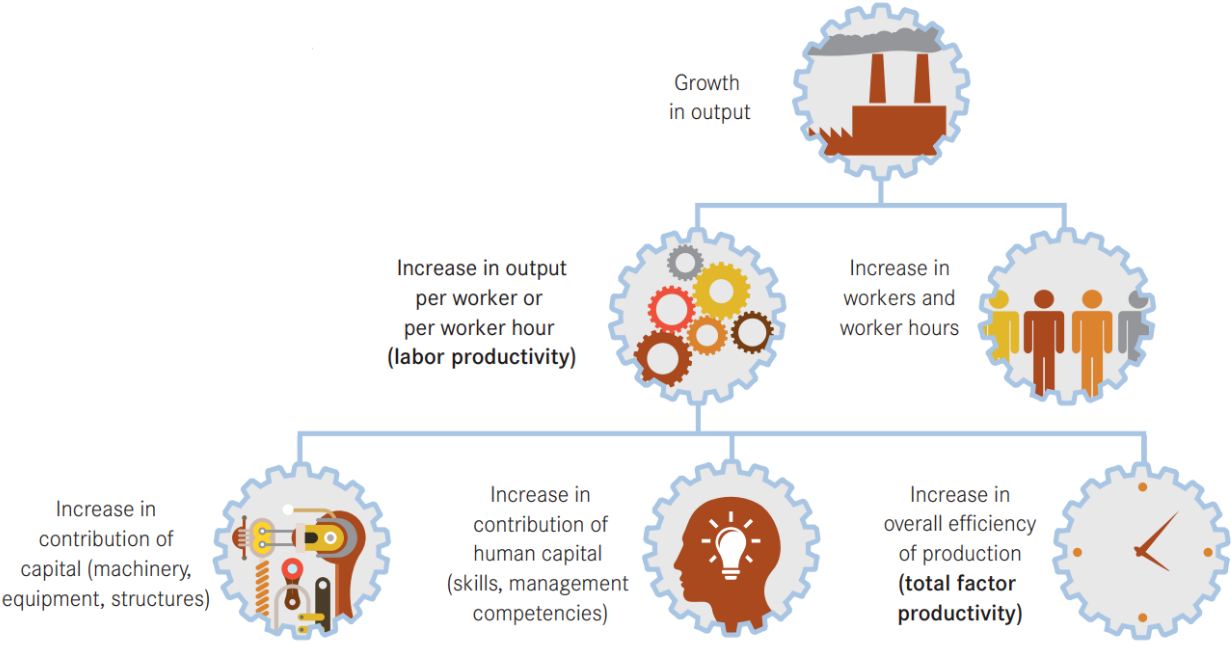
\includegraphics[width=4.16667in,height=4.16667in]{_000_images/003_labor_productivity_total_factor_productivity.png}

}

\caption{\label{fig-labor-factor-productivity-total-factor-productivity}Labor
productivity and total factor productivity
(\citeproc{ref-de_vries_total_2017}{Vries and Azeez Erumban 2017, 21},
fig 3)}

\end{figure}%
\end{frame}

\begin{frame}{}
\phantomsection\label{section-14}
\begin{table}

\caption{\label{tbl-growth-accounting-col}Growth accounting applied to
Colombia for selected years}

\centering{

\centering\begingroup\fontsize{9}{11}\selectfont

\begin{threeparttable}
\begin{tabular}{>{\raggedright\arraybackslash}p{2.5in}rrrr}
\toprule
Measure & 1990 & 2010 & 2020 & 2024\\
\midrule
\cellcolor[HTML]{e31a1c}{Growth in real GDP} & \cellcolor[HTML]{e31a1c}{4.08} & \cellcolor[HTML]{e31a1c}{4.40} & \cellcolor[HTML]{e31a1c}{-7.53} & \cellcolor[HTML]{e31a1c}{2.00}\\
\cellcolor[HTML]{18BC9C}{Contribution of Labor Quantity to real GDP growth} & \cellcolor[HTML]{18BC9C}{1.43} & \cellcolor[HTML]{18BC9C}{1.94} & \cellcolor[HTML]{18BC9C}{-13.53} & \cellcolor[HTML]{18BC9C}{0.66}\\
\cellcolor[HTML]{18BC9C}{Contribution of Labor Quality to real GDP growth} & \cellcolor[HTML]{18BC9C}{0.80} & \cellcolor[HTML]{18BC9C}{1.08} & \cellcolor[HTML]{18BC9C}{1.97} & \cellcolor[HTML]{18BC9C}{0.24}\\
\cellcolor[HTML]{CCBE93}{Contribution of Total Capital Services to real GDP growth} & \cellcolor[HTML]{CCBE93}{1.23} & \cellcolor[HTML]{CCBE93}{2.49} & \cellcolor[HTML]{CCBE93}{0.83} & \cellcolor[HTML]{CCBE93}{1.78}\\
\cellcolor[HTML]{FF7F00}{Growth of Total Factor Productivity} & \cellcolor[HTML]{FF7F00}{0.63} & \cellcolor[HTML]{FF7F00}{-1.12} & \cellcolor[HTML]{FF7F00}{3.20} & \cellcolor[HTML]{FF7F00}{-0.69}\\
\bottomrule
\end{tabular}
\begin{tablenotes}
\item Source: Total Economy Database - Growth Accounting and Total Factor Productivity
\item Last update: 2024
\end{tablenotes}
\end{threeparttable}
\endgroup{}

}

\end{table}%
\end{frame}

\section{Proximate and fundamental determinants of economic
growth}\label{proximate-and-fundamental-determinants-of-economic-growth}

\begin{frame}{}
\phantomsection\label{section-15}
\begin{itemize}
\item
  Proximate determinants

  \begin{itemize}
  \tightlist
  \item
    Increase in workers and worked hours
  \item
    Increase in produced non-financial fixed assets
  \item
    Increase in educational attainment, experience and skills (lifelong
    learning)
  \item
    Increase in overall efficiency of production (total factor
    productivity)
  \end{itemize}
\end{itemize}
\end{frame}

\begin{frame}{}
\phantomsection\label{section-16}
\begin{itemize}
\item
  Fundamental determinants

  \begin{itemize}
  \tightlist
  \item
    Better institutions
    (\citeproc{ref-cardenas_introduccion_2020}{Cardenas 2020, chap. 4})
  \item
    Integration into the global economy
    (\citeproc{ref-cardenas_introduccion_2020}{Cardenas 2020, chap. 5})
  \item
    Geographical conditions
  \end{itemize}
\end{itemize}
\end{frame}

\section{Acknowledgments}\label{acknowledgments}

\begin{frame}{}
\phantomsection\label{section-17}
\begin{itemize}
\item
  To my family that supports me
\item
  To the taxpayers of Colombia and the
  \href{https://www.umng.edu.co/estudiante}{\textbf{UMNG students}} who
  pay my salary
\item
  To the \href{https://www.business-science.io/}{\textbf{Business
  Science}} and \href{https://www.rfordatasci.com/}{\textbf{R4DS Online
  Learning}} communities where I learn
  \href{https://www.r-project.org/about.html}{\textbf{R}} and
  \href{https://www.python.org/about/}{\textbf{\(\pi\)-thon}}
\item
  To the \href{https://www.r-project.org/contributors.html}{\textbf{R
  Core Team}}, the creators of
  \href{https://rstudio.com/products/rstudio/}{\textbf{RStudio IDE}},
  \href{https://quarto.org/}{\textbf{Quarto}} and the authors and
  maintainers of the packages
  \href{https://CRAN.R-project.org/package=tidyverse}{\textbf{tidyverse}},
  \href{https://CRAN.R-project.org/package=knitr}{\textbf{knitr}},
  \href{https://CRAN.R-project.org/package=janitor}{\textbf{janitor}},
  \href{https://CRAN.R-project.org/package=kableExtra}{\textbf{kableExtra}},
  and
  \href{https://CRAN.R-project.org/package=tinytex}{\textbf{tinytex}}
  for allowing me to access these tools without paying for a license
\item
  To the \href{https://www.kernel.org/category/about.html}{\textbf{Linux
  kernel community}} for allowing me the possibility to use some
  \href{https://static.lwn.net/Distributions/}{\textbf{Linux
  distributions}} as my main
  \href{https://en.wikipedia.org/wiki/Operating_system}{\textbf{OS}}
  without paying for a license
\end{itemize}
\end{frame}

\section*{References}\label{references}
\addcontentsline{toc}{section}{References}

\begin{frame}[allowframebreaks]{References}
\phantomsection\label{refs}
\begin{CSLReferences}{1}{0}
\bibitem[\citeproctext]{ref-bolt_maddison_2024}
Bolt, Jutta, and Jan Luiten Van Zanden. 2024a. {``Maddison {Project}
{Database} 2023.''} DataverseNL. \url{https://doi.org/10.34894/INZBF2}.

\bibitem[\citeproctext]{ref-bolt_maddisonstyle_2024}
---------. 2024b. {``Maddison‐style Estimates of the Evolution of the
World Economy: {A} New 2023 Update.''} \emph{Journal of Economic
Surveys}, April, 1--41. \url{https://doi.org/10.1111/joes.12618}.

\bibitem[\citeproctext]{ref-cardenas_introduccion_2020}
Cardenas, Mauricio. 2020. \emph{Introducción a La {Economía}
{Colombiana}}. 4th ed. Alfaomega.

\bibitem[\citeproctext]{ref-nasa_earth_observatory_korea_2012}
Observatory, NASA Earth, Jesse Allen Allen, and Robert Simmon. 2012.
{``Korea and the {Yellow} {Sea}.''}
\url{https://earthobservatory.nasa.gov/images/79796/korea-and-the-yellow-sea}.

\bibitem[\citeproctext]{ref-oecd_measuring_2001}
OECD. 2001. \emph{Measuring {Productivity} - {OECD} {Manual}:
{Measurement} of {Aggregate} and {Industry}-Level {Productivity}
{Growth}}. OECD. \url{https://doi.org/10.1787/9789264194519-en}.

\bibitem[\citeproctext]{ref-oecd_measuring_2009}
---------. 2009. \emph{Measuring {Capital} - {OECD} {Manual} 2009:
{Second} Edition}. OECD. \url{https://doi.org/10.1787/9789264068476-en}.

\bibitem[\citeproctext]{ref-roser_economic_2013}
Roser, Max. 2013. {``Economic {Growth}.''} \emph{Our World in Data},
November. \url{https://ourworldindata.org/economic-growth}.

\bibitem[\citeproctext]{ref-taylor_26_2013}
Taylor, Alan. 2013. {``26 {Years} of {Growth}: {Shanghai} {Then} and
{Now} - {The} {Atlantic}.''}
\url{https://www.theatlantic.com/photo/2013/08/26-years-of-growth-shanghai-then-and-now/100569/}.

\bibitem[\citeproctext]{ref-de_vries_total_2017}
Vries, Klaas de, and Abdul Azeez Erumban. 2017. {``Total {Economy}
{Database}: {A} Detailed Guide to Its Sources and Methods.''}
\url{https://conference-board.org/data/economydatabase/total-economy-database-methodology}.

\end{CSLReferences}
\end{frame}




\end{document}
